\documentclass{article}
\usepackage{graphicx}
\graphicspath{ {./images/} }
\usepackage{fontspec}
\usepackage{polyglossia}
\usepackage{amsmath}
\usepackage{float}
\setmainlanguage{hebrew}
\setmainfont{Times New Roman}
% \newfontfamily{\hebrewfont}{New Peninim MT}
\renewcommand*{\thesection}{}
\renewcommand*{\thesubsection}{\alph{subsection}.}
\renewcommand*{\thesubsubsection}{\arabic{subsubsection}.}
\title{תרגיל בית 1}
\date{}
\begin{document}
\maketitle
\newpage
\section{שאלה 1}
\subsection*{2}
נגדיר את מרחב החיפוש 
$(S, O, I, G)$.
\begin{itemize}
\item[$S$:]
קבוצת המצבים במרחב מייצגים את מיקום הסוכן ואילו כדורי דרקון נאספו. לכן כל מצב מוגדר ע"י מספר התא בו נמצא הסוכן והאם כדור 1 או 2 נאספו.
$$S = ([63]\cup\{0\}) \times \{0,1\} \times \{0, 1\}$$
\item[$O$:]
$$O = \{Down, Up, Left, Right\}$$
\item[$I$:]
$$I = \{(0, False, False)\}$$
\item[$G$:]
$$G = \{(63, True, True)\}$$
\end{itemize}
גודל מרחב המצבים הוא
$$64 \times 2 \times 2 = 256$$

\subsection*{3}
ניתן להפעיל Up בכל מצב חוץ מבחור, לכן הפונקציה Domain על אופרטור Up מוגדרת:
$$Domain(Up) = \{s \in S| board(s[0]) \neq H\}$$
כאשר board הוא לוח המשחק שמיוצג ע"י מחרוזת באורך 64.

\subsection*{4}
מהמצב ההתחלתי ניתן או לנסות לנוע למעלה או שמאלה ואז להישאר במקום, או לנוע ימינה למצב 1, או לנוע למטה למצב 8. לכן
$$Succ(0) = \{0, 1, 8\}$$

\subsection*{5}
במרחב החיפוש שלנו אכן קיימים מעגלים. לדוגמה ניתן ממצב 0 לנוע ימינה למצב 1, ואז לנוע שמאלה למצב 0 ולסגור מעגל.
\subsection*{6}
מקדם הסיעוף בבעיה הוא 4 כיוון שממצב מסוים ניתן לנוע לכל היותר לארבעה מצבים שונים (ויש מצב בו ניתן לנוע לארבעה מצבים שונים, למשל מצב 9).
\subsection*{7}
במקרה הגרוע ביותר, סוכן כללי לא יגיע למצב הסופי. למשל יכול להיות סוכן שנתקע במעגל לנצח.
\subsection*{8}
במקרה הטוב ביותר ידרשו לסוכן 16 פעולות. ראינו בקורס באלגוריתמים ש-BFS מחזיר את המסלול הקצר ביותר במרחב החיפוש, לכן BFS מחזיר את המספר המינימלי של פעולות הנדרש לסוכן כדי להגיע למצב הסופי. נריץ BFS ונקבל שהסוכן מגיע למטרה תוך 16 פעולות.
\subsection*{9}
דוגמה נגדית:
\begin{figure}[h]
	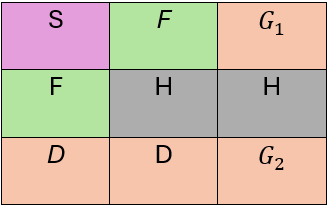
\includegraphics[scale=0.5]{1_9}
\end{figure}
\begin{align*}
&dist_{manhatan}(S,G_1) = 2\\
&dist_{manhatan}(S,G_2) = 4
\end{align*}
המסלול הקל ביותר הוא 
$[Down, Down, Right, Right]$.
מסלול זה אינו מגיע למצב המטרה שהכי קרוב למצב ההתחלתי, בסתירה לטענה.

\section{שאלה 2}
\section{שאלה 3}
\subsection*{1}
האלגוריתם שלם אך לא קביל.
שלמות: מפני שיש מספר סופי של מצבים ומבצעים חיפוש גרף, נובע שיש חסם למספר המצבים במסלול. כלומר חסם עומק L כלשהו. ראינו בתרגול ש-DFS עם חסם עומק L כאשר יש פתרון שאורכו קצר או שווה ל-L הוא שלם.\\
לא קביל:  נסתכל על הלוח
\begin{figure}[H]
	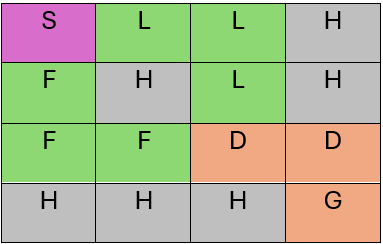
\includegraphics[scale=0.5]{3_1}
\end{figure}
DFS-G
יחזיר את המסלול 
$[0, 0, 1, 1, 1, 0]$
בעוד שהמסלול הקל ביותר הוא
$[1, 1, 0, 0, 1, 0]$.
\subsection*{2}
אלגוריצם DFS על עץ לא בהכרח ימצא פתרון על לוח NxN כללי. לדוגמה ייתכן שהוא יתקע במעגל:
\begin{figure}[H]
	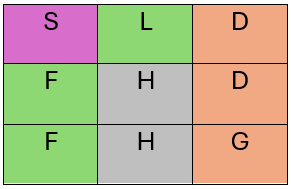
\includegraphics[scale=0.5]{3_2}
\end{figure}
אלגוריתם DFS ינסה לנוע למטה תמיד אם אפשר, לכן הוא יבצע:
$[Down,Down, Up, Down, Up, Down, ...]$
\subsection*{3}
$$Expand = 2N - 2$$
$$Create = 4N-4$$
הסוכן קודם כל ינסה לבצע Down ולאחר מכן Right.
לכן האלגוריתם יבצע: Down עד הגעה לקיר התחתון ואז Right עד הגעה למטרה. עבור לוח כללי 
$N\times N$:
\begin{figure}[H]
	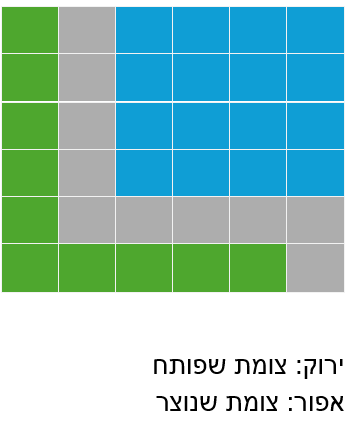
\includegraphics[scale=0.5]{3_3}
\end{figure}
\subsection*{4}
במהלך חיפוש 
BFS-G backtracking
יפותחו אותו מספר צמתים כמו ב-DFS-G כלומר
$2N-2$
ומפני שנוצרים צמתים בצורה עצלה, נובע שיווצרו גם כן
$2N-2$
צמתים.
\section{שאלה 7}
נסמן מצב כללי ב-
$s = (s_x, s_y)$,
ואת המצב הסופי ב-
$g = (g_x, g_y)$.
בנוסף נגדיר
$$x := |s_x - g_x|$$
$$y := |s_y - g_y|$$
נשים לב כי המסלול הזול ביותר האפשרי בין מצב כללי למצב הסופי, הוא מסלול שעובר דרך כביש שמחבר את שתי הנקודות, כלומר
$$\sqrt{x^2+y^2} = dist(s,g) \leq h^*(s)$$
\subsection*{1}
האפסילון ההדוק ביותר המקיים זאת הוא
$\epsilon = \sqrt{2}$.\\\\
יהי
$s \in S$.
נחלק למקרים:
\begin{itemize}
\item[$s=g$:]
$$0 = \epsilon \cdot h_{MD}(s) \leq h^*(s) = 0$$
\item[$s\neq g$:]
נשים לב כי
$$x^2 + y^2 - 2xy = (x-y)^2 \geq 0 \rightarrow x^2 + y^2 \geq 2xy$$
ולכן
$$\frac{2xy}{(x^2+y^2)} \leq 1$$
$$\frac{h(s)}{dist(s,g)} = \sqrt{\frac{(x+y)^2}{(x^2+y^2)}} = \sqrt{\frac{x^2+y^2+2xy}{(x^2+y^2)}}=\sqrt{1+\frac{2xy}{(x^2+y^2)}}\leq \sqrt{2}$$
$$h(s) \leq \sqrt{2}dist(s,g) \leq \sqrt{2}h^*(s) = \epsilon \cdot h^*(s)$$
שוויון מתקבל עבור 
$x=y$
כאשר יש כביש ישיר שמחבר בין הנקודות. במצב זה מתקיים
$$\sqrt{2x^2} = dist(s,g) = h^*(s)$$
לכן
$$h(s) = 2x = \sqrt{2}\cdot \sqrt{2x^2} = \epsilon \cdot dist(s,g) = \epsilon \cdot h^*(s)$$
\end{itemize}
\subsection*{2}
האפסילון ההדוק ביותר המקיים זאת הוא 
$\epsilon = 1$.\\
$$h(s) = min\{x,y\} \leq \sqrt{x^2+y^2} = dist(s,g) \leq  h^*(s)$$
שיוויון מתקבל עבור 
$x = 0$
וכאשר יש כביש שמחבר ישירות בין שתי הנקודות:
$$h(s) = y = dist(s,g) = h^*(s)$$
\section{שאלה 9}
\subsection*{2}
\begin{itemize}
\item[(a]
לא נכון. עבור 
$w_1 = 0, \quad w_2 = 1$.
נסמן
\begin{align*}
&f_1 = g \cdot w_1 = g\\
&f_2 = g \cdot w_2 = g + h
\end{align*}
הרצת 
$W-A*$
עם
$f_1$
שקול ל-UCS שמחזיר מסלול אופטימלי.\\
הרצת 
$W-A*$
עם
$f_2$
שקול ל-A* שמחזיר מסלול אופטימלי (כי היוריסטיקה קבילה).\\
לכן
$$cost(p_1) = cost(p_2)$$
בסתירה לטענה.
\item[(b]
הראינו כי הטענה לא נכונה עבור יוריסטיקה קבילה, ולכן גם אינה נכונה עבור יוריסטיקה כללית.
\end{itemize}
\section{שאלה 11}
\subsection*{2}
יתרון:יעיל יותר חישובית.\\
חיסרון: לא מובטח פתרון אופטימלי, לעומת A* שבהינתן יוריסטיקה קבילה מבטיח פתרון אופטימלי.
\subsection*{3}
הצעה ליוריסטיקה:\\
D
היא קבוצת כדורי הדרקון,
$D = \{d1, d2\}$.
$$h_{dist}(s) = min\{h_{euclidean}(s,g)| g \in G \cup D\}$$
\begin{figure}[H]
	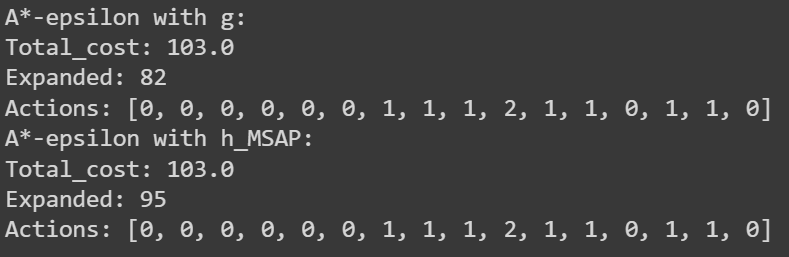
\includegraphics[scale=0.5]{11_3}
\end{figure}
ניתן לראות שהמסלולים זהים, אך כמות הצמתים שפותחו עבור
$h_{Focal}=h_{MSAP}$
גדול יותר.
\subsection*{4}
התנהגות האלגוריתם תהיה כמו greedy לפי 
$h_{Focal}$.\\
אם נגדיר את אפסילון שווה לאינסוף, אזי נקבל
$$Focal = \{n\in OPEN | f(n) \leq \inf\} = OPEN$$ 
ואז נבחר את הצומת
$$min_{n \in Focal} h_{Focal}(n) = min_{n \in OPEN} h_{Focal}(n)$$
כלומר נבחר את הצומת מ-Open עם ערך 
$h_{Focal}$
המינימלי.
\section{שאלה 13}
\subsection*{1}
$$p(b|a) = \frac{2}{5}, \quad p(c|a) = \frac{2}{5}, \quad p(d|a) = \frac{1}{5}$$
\subsection*{2}
נשים לב שהאלגוריתם יכול לעבור רק לצמתים עם ערך גדול ממש. לכן נחפש מסלול ארוך ביותר שהערכי הצמתים בו עולים ממש.
מספר הצעדים המקסימלי שהאלגוריתם יכול לבצע תלוי בערך של 
$\beta$.\\
שלושה צעדים אם 
$\beta > 4$:
$A \rightarrow B \rightarrow F \rightarrow G$.\\
שני צעדים אם 
$\beta \leq 4$:
$A \rightarrow B \rightarrow G$.
\subsection*{3}
האלגוריתם לא יתכנס למקסימום הגלובלי, בהינתן שבצעד הראשון האלגוריתם עבר למצב C$.$ ממצב C ניתן לעבור רק ל-H מפני שמצב B בעל ערך שווה ל-C$.$ לכן האלגוריתם יתכנס למצב H שערכו 3 בעוד שהמקסימום הגלובלי הוא
$max\{4, \beta\}$.
\subsection*{4}
ההסתברות שהאלגוריתם יתכנס לפתרון לא אופטימלי:
$$\left\{\begin{array}{ll}
\frac{3}{5},& \quad \beta \geq 4\\
1-\frac{2}{5}\cdot \frac{\beta-2}{\beta},& \quad \beta < 4
\end{array}\right.$$
נשים לב שבכל מקרה אם נגיע ל-C או D אז לא נתכנס לפתרון גלובלי. לכן בשתי האפשרויות נרצה קודם להגיע ל-B$.$ ההסתברות לכך היא 
$p(b|a)$.\\
במקרה הראשון הפתרון האופטימלי הוא G ולכן מספיק להגיע אל B כי מ-B לבסוף נתכנס לפתרון אופטימלי: או שנעבור ישירות ל-G או שנעבור ל-F ואז ל-G$.$\\
במקרה השני הפתרון האופטימלי הוא F ולכן נדרוש שנגיע ל-B ואז ל-F$.$ ההסתברות לכך היא 
$p(b|a) \cdot p(f|b) = \frac{2}{5} \cdot \frac{\beta-2}{\beta}$.
\subsection*{5}
אף 
$\beta$
לא מקיים זאת. ראינו בסעיף 2 שרק אם 
$\beta > 4$
אז קיים מסלול באורך שלושה צעדים אל המקסימום הגלובלי, ושמסלול זה הוא
$A \rightarrow B \rightarrow F \rightarrow G$.\\
ההסתברות לעבור במסלול זה היא
$$p(b|a) \cdot p(f|b) \cdot p(g|f) = \frac{2}{5} \cdot \frac{4-2}{4-2 + \beta-2} \cdot 1 = \frac{4}{5\beta}$$
נדרוש שההסתברות לכך תהיה גדולה מחמישית:
$$\frac{4}{5\beta} > \frac{1}{5}$$
לכן
$$\beta < 4$$
סתירה.
\end{document}